\documentclass{standalone}
\usepackage{tikz}
\usepackage{amsmath}
\usetikzlibrary{shapes.geometric, arrows, calc}
\usepackage{textcomp}
\usepackage{comment}
%\usetikzlibrary{external} 
%\tikzexternalize[prefix=tikz/]

\tikzstyle{startstop} = [rectangle, rounded corners, 
minimum width=3cm, 
minimum height=1cm,
text centered, 
draw=black, 
fill=red!30]

\tikzstyle{io} = [trapezium, 
trapezium stretches=true, % A later addition
trapezium left angle=70, 
trapezium right angle=110, 
minimum width=3cm, 
minimum height=1cm, 
%text centered, 
align=center,
draw=black, fill=blue!30]

\tikzstyle{process} = [rectangle, 
minimum width=6cm, 
minimum height=1cm, 
text centered, 
text width=5cm, 
draw=black, 
fill=orange!30]

\tikzstyle{process_left} = [rectangle, 
minimum width=6cm, 
minimum height=1cm, 
%text centered, 
text width=5cm, 
draw=black, 
fill=orange!30]

\tikzstyle{process_wider} = [rectangle, 
minimum width=8cm, 
minimum height=1cm, 
%text centered, 
text width=7cm, 
draw=black, 
fill=orange!30]

\tikzstyle{process_wide} = [rectangle, 
minimum width=13cm, 
minimum height=1cm, 
%text centered, 
text width=12cm, 
draw=black, 
fill=orange!30]

\tikzstyle{decision} = [diamond, 
minimum width=3cm, 
minimum height=1cm, 
%text centered, 
align=center, % text centered does not allow multiline text
draw=black, 
fill=green!30]
\tikzstyle{arrow} = [thick,->,>=stealth]
\begin{document}

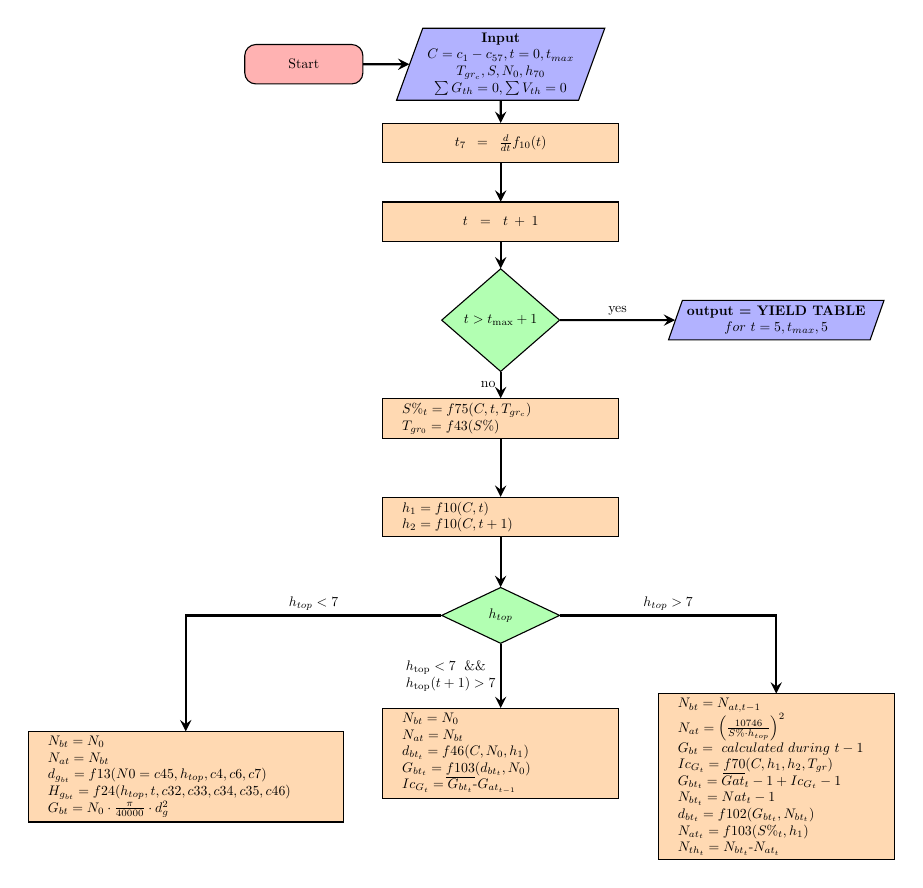
\begin{tikzpicture}[node distance=2cm, scale=0.5, transform shape]
%\begin{tikzpicture}[node distance=2cm, transform shape]

\node (start) [startstop] {Start};
\node (in1) [io, right of=start, xshift=3cm] {
\textbf{Input} \\
$ C = c_1-c_{57} , t=0, t_{max}$  \\
$ T_{gr_{c}} , S, N_0 , h_{70} $ \\
$ \sum G_{th} = 0, \sum V_{th} = 0 $
};
\draw [arrow] (start) -- (in1);

\node (pro0) [process, below of=in1] {
$t_7=\frac{d}{dt} f_{10}(t)$
};
\draw [arrow] (in1) -- (pro0);

\node (pro1) [process, below of=pro0] {$t=t+1$};
\draw [arrow] (pro0) -- (pro1);

% Eerste beslissing
\node (dec1) [decision, below of=pro1, yshift=-0.5cm] {$t>t_{\text{max}}+1$};
\node (out0) [io, right of=dec1, xshift=5cm] {
\textbf{output = YIELD TABLE} \\
$for \ t = 5, t_{max}, 5$
};
\draw [arrow] (pro1) -- (dec1);

\node (pro2) [process_left, below of=dec1, yshift=-0.5cm] {
$S\%_t=f75(C, t, T_{gr_{c}} )$ \\
$T_{gr_{0}}=f43(S\%)$
};
\node (pro3) [process_left, below of=pro2, yshift=-0.5cm] {
$h_1 = f10(C, t)$\\
$h_2 = f10(C, t+1)$
};
\draw [arrow] (dec1) -- node[anchor=east] {no} (pro2);
\draw [arrow] (dec1) -- node[anchor=south] {yes} (out0);
\draw [arrow] (pro2) -- (pro3);




% 5. Tweede beslissing
\node (dec2) [decision, below of=pro3, yshift=-0.5cm] {$h_{top}$};
\draw [arrow] (pro3) -- (dec2);


\node (proces_htop_lt_7) [process_wider, left of=dec2, xshift=-6cm, yshift=-4.1cm] {
$N_{bt} = N_0$ \\
$N_{at} = N_{bt}$ \\
$d_{g_{bt}} = f13(N0=c45, h_{top}, c4, c6, c7)$ \\
$H_{g_{bt}} = f24(h_{top}, t, c32, c33, c34, c35, c46)$ \\
$G_{bt} = N_0 \cdot \frac{\pi}{40000} \cdot d_g^2$ \\
};
% \draw [arrow] (dec2) -- node[anchor=west, midway, above] {$h_{top}<7} (proces_htop_lt_7);
% \draw [arrow] (dec2)  -| node[anchor=west, midway, above] {$h_{top}<7$} (proces_htop_lt_7);
\draw [arrow] (dec2) -| node[pos=0.25, above] {$h_{top} < 7$} (proces_htop_lt_7);

% 6a
\node (proces_htop_eq_7) [process_left, below of=dec2, yshift=-1.5cm] {
$N_{bt} = N_0$ \\
$N_{at} = N_{bt}$ \\
$d_{bt_{t}} = f46(C, N_0 , h_1)$ \\
$G_{bt_{t}} = \underline{f103}(d_{bt_{t}} , N_0 )$ \\
$Ic_{G_{t}} = G_{bt_{t}}\text{-}G_{at_{t-1}}$
};
% \draw [arrow] (dec2) -- node[anchor=south, midway, left] 
%     {$h_{\text{top}} < 7$ \\ $h_{\text{top}} > 7$}
%     (proces_htop_eq_7);
\draw [arrow] (dec2) -- node[anchor=south, midway, left, align=left] 
{$h_{\text{top}} < 7$ \;\&\&\; \\ $h_{\text{top}}(t+1) > 7$} (proces_htop_eq_7);



% 6b
\node (proces_htop_gt_7) [process_left, right of=dec2, xshift=5cm, yshift=-4.1cm] {
$N_{bt} = N_{at, t-1}$ \\
$N_{at} = \left(\frac{10746}{S\% \cdot h_{top}}\right)^2$ \\
$G_{bt} = \ calculated\ during\ t-1 $\\
$Ic_{G_{t}} = \underline{f70}(C, h_1 , h_2, T_{gr})$ \\
$G_{bt_{t}} = Gat_t-1+Ic_{G_{t}}-1$ \\
$N_{bt_{t}} = Nat_t-1$ \\
$d_{bt_{t}} = f102(G_{bt_{t}} , N_{bt_{t}} )$ \\
$N_{at_{t}} = f103(S\%_t , h_1)$ \\
$N_{th_{t}} = N_{bt_{t}}\text{-}N_{at_{t}}$
};
% \draw [arrow] (dec2) -- node[anchor=east, midway, above] {yes} (proces_htop_gt_7);
\draw [arrow] (dec2) -| node[pos=0.25, above] {$h_{top} > 7$} (proces_htop_gt_7);




% \draw [arrow] (out0) -- (stop);


\begin{comment}
% 7. Derde beslissing
\node (dec3) [decision, below of=pro4, yshift=-2cm] {
$ N_{th_{t}}>0$ \\
$ t = 5, 120 , 5$
};

% 8a.
\node (pro6) [process_left, below of=pro5, yshift=-2.5cm] {$
N_{bt_{t}} = N_{at_{t-1}}, N_{at_{t}} = N_{bt_{t}},  G_{at_{t}} = G_{bt_{t}}, N_{th_{t}} = 0  G_{th_{t}} = 0, d_{th_{t}} = 0
$};
\node at ($(pro6.north) + (-1cm, 0)$) (north1) {};
\node at ($(pro6.north) + (1cm, 0)$) (north2) {};
% 8b
\node (pro7) [process_left, below of=dec3, yshift=-1.25cm] {
$d_{at_{t}} = \underline{f86}(d_{bt_{t}}, h_1, h_{70}, t, T_{gr_{0}})$  \\
$G_{at_{t}} = \underline{f103}(d_att, N_att )$ \\
$G_{th_{t}} = G_{b_{tt}}\text{-}G_{at_{t}}$ \\
$d_{th_{t}} = f102(G_{th_{t}}, N_{th_{t}})$
};
\draw [arrow] (pro5) -- (pro6);
\draw [arrow] (pro4) -- (dec3) ;
\draw [arrow, shorten >=-1mm] (dec3.west)  -| node[anchor=west, midway, above] {no} (north2);
\draw [arrow] (dec3) -- node[anchor=northi, right]{yes} (pro7);

% Laatste vak
\node (pro8) [process_wide, below of=pro6, yshift=-2.75cm, xshift=3.5cm] {
$ h_{top_{t}} = h_1; hdom_t = \underline{f87}(C, h_1, N_{at_{t}}); d_{dom_{t}} = \underline{f88}(C, d_{at_{t}}, h_{70} , T_{gr_{0}})$\\
$ h_{at_{t}} = \underline{f89}(C, t, h_{70}, T_{gr_{0}}); h_{bt_{t}} = \underline{f90}(C, h_{at_{t}})$\\
$ for\ h_1\leq 7: \ V_{bt_{t}} = N_{bt_{t}}\cdot \underline{f91}(C, d_{bt_{t}}, h_{bt_{t}})$ \\
$ \qquad\qquad\qquad V_{at_{t}} = N_{at_{t}} \cdot \underline{f91}(C, d_{at_{t}} , h_{at_{t}})$\\
$ for\ h_1>7: V_{bt_{t}} = f93(C, G_{bt_{t}} , h_1 )$ \\
$ \qquad\qquad\qquad V_{at_{t}} = f93(C, G_{at_{t}} , h_1 )$ \\
$ V_{th_{t}} = V_{bt{t}} - V_{at_{t}} ; \sum G_{th_{t}} = \sum G_{th_{t - 1}}+G_{th_{t}} $ \\
$ \sum V_{th_{t}} = \sum V_{th_{t-1}}+V_{th{t}}$  \\
$ G_{tot_{t}} = G_{at_{t}}+ \sum G_{th_{t}} ; V_{tot_{t}} = V_{at_{t}}+ \sum V_{th_{t}} $ \\
$ Im_{G_{t}} = G_{tot_{t}} /t; Im_{V_{t}} = V_{tot_{t}} /t $ \\
$ Ic_{G{t-1}} = (G_{tot_{t}}-G_{tot_{t-2}})/2; Ic{V{t-1}} = (V_{tot_{t}}-V_{tot_{t-2}})/2 $ 
};
\node at ($(pro8.north) + (-3.5cm, 0)$) (north81) {};
\node at ($(pro8.north) + (3.5cm, 0)$) (north82) {};
\draw [arrow, shorten >=-1mm] (pro6) -- (north81);
\draw [arrow, shorten >=-1mm] (pro7) -- (north82);

\draw [arrow] (pro8.west) -- ++(-2, 0) -- ++(0, 21.75) -- (pro1.west);


\node (stop) [startstop, below of=out0] {Stop};

\draw [arrow] (start) -- (in1);
\draw [arrow] (start) -- (in1);
\draw [arrow] (in1) -- (pro0);
\draw [arrow] (pro0) -- (pro1);
\draw [arrow] (pro1) -- (dec1);
\draw [arrow] (dec1) -- node[anchor=east] {no} (pro2);
\draw [arrow] (dec1) -- node[anchor=south] {yes} (out0);
\draw [arrow] (pro2) -- (pro3);
\draw [arrow] (pro3) -- (dec2);
\draw [arrow] (out0) -- (stop);
\end{comment}

\end{tikzpicture}
\end{document}
